\documentclass[cic,tc]{iiufrgs}
\usepackage[utf8]{inputenc}   % pacote para acentuação
\usepackage{graphicx}         % pacote para importar figuras
\usepackage{times}            % pacote para usar fonte Adobe Times
% \usepackage{palatino}
% \usepackage{mathptmx}       % p/ usar fonte Adobe Times nas fórmulas
\usepackage[alf,abnt-emphasize=bf]{abntex2cite}	% pacote para usar citações abnt

%
% Informações gerais
%
\title{Estudo e otimização dos softwares de análise filogenética do Hospital de
Clínicas de Porto Alegre}

\author{Farah}{Alef}
% alguns documentos podem ter varios autores:
% \author{Flaumann}{Frida Gutenberg}
% \author{Flaumann}{Klaus Gutenberg}

% orientador e co-orientador são opcionais (não diga isso pra eles :))
\advisor[Prof.~Dr.]{Geyer}{Claudio Fernando Resin}
\coadvisor[Prof.~Dr.]{Anjos}{Julio Cesar Santos}

% a data deve ser a da defesa; se nao especificada, são gerados
% mes e ano correntes
\date{novembro}{2021}

% o local de realização do trabalho pode ser especificado (ex. para TCs)
% com o comando \location:
\location{Porto Alegre}{RS}

% itens individuais da nominata podem ser redefinidos com os comandos
% abaixo:
% \renewcommand{\nominataReit}{Prof\textsuperscript{a}.~Wrana Maria Panizzi}
% \renewcommand{\nominataReitname}{Reitora}
% \renewcommand{\nominataPRE}{Prof.~Jos{\'e} Carlos Ferraz Hennemann}
% \renewcommand{\nominataPREname}{Pr{\'o}-Reitor de Ensino}
% \renewcommand{\nominataPRAPG}{Prof\textsuperscript{a}.~Joc{\'e}lia Grazia}
% \renewcommand{\nominataPRAPGname}{Pr{\'o}-Reitora Adjunta de P{\'o}s-Gradua{\c{c}}{\~a}o}
% \renewcommand{\nominataDir}{Prof.~Philippe Olivier Alexandre Navaux}
% \renewcommand{\nominataDirname}{Diretor do Instituto de Inform{\'a}tica}
% \renewcommand{\nominataCoord}{Prof.~Carlos Alberto Heuser}
% \renewcommand{\nominataCoordname}{Coordenador do PPGC}
% \renewcommand{\nominataBibchefe}{Beatriz Regina Bastos Haro}
% \renewcommand{\nominataBibchefename}{Bibliotec{\'a}ria-chefe do Instituto de Inform{\'a}tica}
% \renewcommand{\nominataChefeINA}{Prof.~Jos{\'e} Valdeni de Lima}
% \renewcommand{\nominataChefeINAname}{Chefe do \deptINA}
% \renewcommand{\nominataChefeINT}{Prof.~Leila Ribeiro}
% \renewcommand{\nominataChefeINTname}{Chefe do \deptINT}

% A seguir são apresentados comandos específicos para alguns
% tipos de documentos.

% Relatório de Pesquisa [rp]:
% \rp{123}             % numero do rp
% \financ{CNPq, CAPES} % orgaos financiadores

% Trabalho Individual [ti]:
% \ti{123}     % numero do TI
% \ti[II]{456} % no caso de ser o segundo TI

% Monografias de Especialização [espec]:
% \espec{Redes e Sistemas Distribuídos}      % nome do curso
% \coord[Profa.~Dra.]{Weber}{Taisy da Silva} % coordenador do curso
% \dept{INA}                                 % departamento relacionado

%
% palavras-chave
% iniciar todas com letras minúsculas, exceto no caso de abreviaturas
%
\keyword{análise filogenética}
\keyword{otimização}
\keyword{paralelismo}
%\keyword{}

%\settowidth{\seclen}{1.10~}

%
% inicio do documento
%
\begin{document}

% folha de rosto
% às vezes é necessário redefinir algum comando logo antes de produzir
% a folha de rosto:
% \renewcommand{\coordname}{Coordenadora do Curso}
\maketitle

% dedicatoria
% \clearpage
% \begin{flushright}
%     \mbox{}\vfill
%     {\sffamily\itshape
%       ``If I have seen farther than others,\\
%       it is because I stood on the shoulders of giants.''\\}
%     --- \textsc{Sir~Isaac Newton}
% \end{flushright}

% agradecimentos
%\chapter*{Agradecimentos}
%Agradeço ao \LaTeX\ por não ter vírus de macro\ldots



% resumo na língua do documento
\begin{abstract}
  A análise filogenética compreende o estudo da evolução dos organismos e suas
  características. Neste trabalho foi realizado um estudo e otimização dos
  problemas de desempenho presentes nos softwares de análise filogenética
  utilizados pelo grupo de pesquisa em genética do Hospital de Clínicas de
  Porto Alegre (HCPA), empregando para isso técnicas de processamento paralelo.
  O tempo total da análise realizada pelo grupo foi reduzido de X para Y. % TODO
\end{abstract}

% resumo na outra língua
% como parametros devem ser passados o titulo e as palavras-chave
% na outra língua, separadas por vírgulas
\begin{englishabstract}{Study and optimization of the phylogenetic analysis software used by Hospital de Clínicas de Porto Alegre}{Phylogenetic analysis. Optimization. Parallelism.} Phylogenetic analysis comprises the study of the evolution of living beings and their characteristics. In this paper we studied and optimized the performance bottlenecks present in the phylogenetic analysis software used by the genetics research group from the Hospital de Clínicas de Porto Alegre, using parallel programming techniques. The analysis total execution time was reduced from X to Y. % TODO
\end{englishabstract}

% lista de figuras
\listoffigures

% lista de tabelas
\listoftables

% lista de abreviaturas e siglas
% o parametro deve ser a abreviatura mais longa
\begin{listofabbrv}{SPMD}
    \item[SMP] Symmetric Multi-Processor
    \item[NUMA] Non-Uniform Memory Access
    \item[SIMD] Single Instruction Multiple Data
    \item[SPMD] Single Program Multiple Data
    \item[ABNT] Associação Brasileira de Normas Técnicas
\end{listofabbrv}

% idem para a lista de símbolos
% \begin{listofsymbols}{$\alpha\beta\pi\omega$}
%     \item[$\sum{\frac{a}{b}}$] Somatório do produtório
%     \item[$\alpha\beta\pi\omega$] Fator de inconstância do resultado
% \end{listofsymbols}

% sumario
\tableofcontents

% aqui comeca o texto propriamente dito

% introducao
\chapter{Introdução}

Neste trabalho foi realizado um estudo e otimização dos problemas de desempenho
presentes nos softwares de análise filogenética utilizados pelo grupo de
pesquisa em genética do Hospital de Clínicas de Porto Alegre (HCPA), empregando
para isso técnicas de processamento paralelo e distribuído sempre que viável.

A análise realizada pelo grupo emprega softwares diversos, que apresentavam
tempos de execução proibitivamente lentos - a análise de um único gene levava
até dois dias, enquanto o grupo pretende analisar centenas de genes - além de
uso de memória proibitivamente elevado em certas etapas da análise. Neste
trabalho foram estudados os softwares utilizados pelo grupo, realizando para
tal revisão bibliográfica sobre o tema e análises de desempenho aprofundadas.
Além disso, foi estudada a possibilidade de paralelização dos algoritmos
empregados visando a redução do seu tempo de execução, e, sempre que possível,
foi implementada tal paralelização, seguida de novas análises, tanto da
corretude da nova implementação como das melhorias de desempenho obtidas.

Por fim, as otimizações resultantes deste trabalho nos diversos softwares que
compõem a análise filogenética foram reunidas em uma ferramenta para execução
de ponta a ponta da análise. Com isso, obteve-se uma redução significativa do
tempo total de execução da análise, que de vários dias passou a levar algumas
horas.

A análise filogenética, cujos softwares associados foram objeto de estudo desse
trabalho, compreende o estudo da evolução de um ou mais organismos e suas
características. Para compreender tal análise em mais detalhes, convém primeiro
reforçar alguns conceitos mais básicos de biologia.

\section{Conceitos de biologia}



%\section{Figuras e tabelas}
%
%Esta seção faz referência às Figuras~\ref{fig:estrutura},~\ref{fig:ex1} e~\ref{fig:ex2}, a título de exemplo. A primeira figura apresenta a estrutura de uma figura. A \emph{descrição} deve aparecer \textbf{acima} da figura. Abaixo da figura, deve ser indicado a origem da imagem, mesmo se essa for apenas os autores do texto.
%
%A Figura~\ref{fig:ex1} representa o caso mais comum, onde a figura propriamente dita é importada de um arquivo ( neste exemplo o formato é \texttt{eps} ou \texttt{pdf}. Veja a seção \ref{sec:fig_format}). A Figura~\ref{fig:ex2} exemplifica o uso do environment \texttt{picture}, para desenhar usando o próprio~\LaTeX.
%
%\begin{figure}[h]
%    \caption{Descrição da Figura deve ir no topo}
%    \begin{center}
%        % Aqui vai um includegraphics , um picture environment ou qualquer
%        % outro comando necessário para incorporar o formato de imagem
%        % utilizado.
%        \begin{picture}(100,100)
%            \put(0,0){\line(0,1){100}}
%            \put(0,0){\line(1,0){100}}
%            \put(100,100){\line(0,-1){100}}
%            \put(100,100){\line(-1,0){100}}
%            \put(10,50){Uma Imagem}
%        \end{picture}
%    \end{center}
%    \label{fig:estrutura}
%    \legend{Fonte: Os Autores}
%\end{figure}
%
%\begin{figure}
%    \caption{Exemplo de figura importada de um arquivo e também exemplo de caption muito grande que ocupa mais de uma linha na Lista~de~Figuras}
%    \begin{center}
%        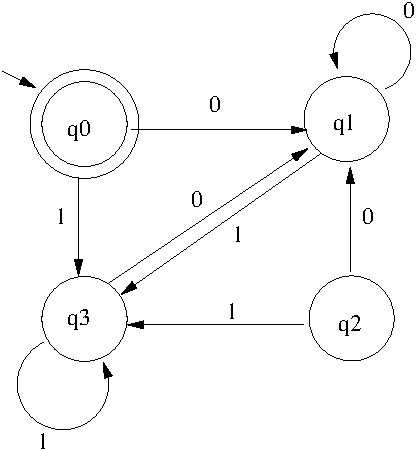
\includegraphics[width=8em]{fig}
%    \end{center}
%    \legend{Fonte: Os Autores}
%    \label{fig:ex1}
%\end{figure}
%
%% o `[h]' abaixo é um parâmetro opcional que sugere que o LaTeX coloque a
%% figura exatamente neste ponto do texto. Somente preocupe-se com esse tipo
%% de formatação quando o texto estiver completamente pronto (uma frase a mais
%% pode fazer o LaTeX mudar completamente de idéia sobre onde colocar as
%% figuras e tabelas)
%% \begin{figure}[h]
%\begin{figure}
%    \caption{Exemplo de figura desenhada com o environment \texttt{picture}.}
%    \begin{center}
%        \setlength{\unitlength}{.1em}
%        \begin{picture}(100,100)
%            \put(20,20){\circle{20}}
%            \put(20,20){\small\makebox(0,0){a}}
%            \put(80,80){\circle{20}}
%            \put(80,80){\small\makebox(0,0){b}}
%            \put(28,28){\vector(1,1){44}}
%        \end{picture}
%    \end{center}
%    \legend{Fonte: Os Autores}
%    \label{fig:ex2}
%\end{figure}
%
%Tabelas são construídas com praticamente os mesmos comandos. Ver a tabela \ref{tbl:ex1}.
%
%\begin{table}[h]
%    \caption{Uma tabela de Exemplo}
%    % OBS: não use \begin{center}, pois este aumenta o espaçamento entre a caption/legend e a tabela
%    % Para figuras, a aparência é melhor com o espaçamento extra
%    \centering
%        \begin{tabular}{c|c|p{5cm}}
%          \hline
%          \textit{Col 1}  &   \textit{Col 2}  &   \textit{Col 3} \\
%          \hline
%          \hline
%          Val 1           &   Val 2           & Esta coluna funciona como um parágrafo, tendo uma margem definida em 5cm. Quebras de linha funcionam como em qualquer parágrafo do tex. \\
%          Valor Longo     & Val 2             & Val 3 \\
%          \hline
%        \end{tabular}
%    \legend{Fonte: Os Autores}
%    \label{tbl:ex1}
%\end{table}
%
%\subsection{Formato de Figuras}
%\label{sec:fig_format}
%
%O LaTeX permite utilizar vários formatos de figuras, entre eles \emph{eps}, \emph{pdf}, \emph{jpeg} e \emph{png}. Programas de diagramação como Inkscape (e mesmo LibreOffice) permitem gerar arquivos de imagens vetoriais que podem ser utilizados pelo LaTeX sem dificuldade. Pacotes externos permitem utilizar SVG e outros formatos.
%
%Dia e xfig são programas utilizados por dinossauros para gerar figuras vetoriais. Se possível, evite-os.
%
%\subsection{Classificação dos etc.}
%
%O formato do instituo de informática define 5 níveis: capítulo, seção, subseção e outros 2 sem nome.
%
%\subsubsection{Subsubseção}
%Exemplo de uma subsubseção.
%
%\paragraph{Parágrafo}
%Exemplo de um parágrafo.

\section{Sobre as referências bibliográficas}

A classe \emph{iiufrgs} faz uso do pacote \emph{abnTeX2} com algumas alterações
feitas por Sandro Rama Fiorini. Culpe ele se algo der errado. Agradeça a ele
pelo que der certo. As modificações dão uma camada de tinta NATBIB-style,
já que o abntex2 usa uns comandos de citação feitos para alienígenas de 5 braços
wtf. Exemplos de citação:

\begin{itemize}
    \item \emph{cite}: Unicórnios são verdes \cite{Adams2009Conceptual};
    \item \emph{citep}:Unicórnios são verdes \citep{Adams2009Conceptual};
    \item \emph{citet}: Segundo \citet{Adams2009Conceptual}, unicórnios são
    verdes.
    \item \emph{citen or citenum}: Segundo \citen{Adams2009Conceptual},
    unicórnios são verdes.
    \item \emph{citeauthor e citeyearpar}: Segundo artigos de
    \citeauthor{Adams2009Conceptual} , unicórnios são verdes
    \citeyearpar{Adams2009Conceptual}.

\end{itemize}

O estilo abnt fornecido antigamente pelo UTUG não é mais recomendado, pois não
produz saída de acordo com as exigências da biblioteca.

Recomenda-se o uso de bibtex para gerenciar as referências (veja o arquivo
biblio.bib).

\section{Mais uma Seção}

Agora vamos fazer várias seções para termos valores de 2 dígitos no \contentsname.

\section{Mais uma Seção}
\section{Mais uma Seção}
\section{Mais uma Seção}
\section{Mais uma Seção}
\section{Mais uma Seção}
\section{Mais uma Seção}
\section{Mais uma Seção}
\section{Mais uma Seção}
\section{Mais uma Seção}


% e aqui vai a parte principal
%
% \chapter{Estado da arte}
% \chapter{Mais estado da arte}
% \chapter{A minha contribuição}
% \chapter{Prova de que a minha contribuição é válida}
% \chapter{Conclusão}

% referências
% aqui será usado o environment padrao `thebibliography'; porém, sugere-se
% seriamente o uso de BibTeX e do estilo abnt.bst (veja na página do
% UTUG)
%
% observe também o estilo meio estranho de alguns labels; isso é
% devido ao uso do pacote `natbib', que permite fazer citações de
% autores, ano, e diversas combinações desses

\bibliographystyle{abntex2-alf}
\bibliography{biblio}

\end{document}
